\chapter{方法间的多模态融合策略探究}
\label{cha:fStrategy}

本章主要介绍方法内以及方法间的多模态融合策略探究,包括其融合思想、操作步骤和实验结果。融合策略在多模态信息利用理解中起着举足轻重的作用,优秀的融合策略可以提高处理的效率(降低时间复杂度),降低成本(降低空间复杂度),更好地利用相辅相成的数据以及方法之间的互补性,弥补不同模态以及方法的不足。在分类、决策、识别等任务中获得更好的效果(提高准确率和鲁棒性)。好的融合策略往往还具备更高的可拓展性。
在本章,我们首先利用传统的分层匹配追踪,以及随机权值卷积递归神经网络来进行颜色和深度信息的提取和融合,并探究不同模态的信息之间的互补性。然后我们在这两种方法的基础上而引入了不同方法之间融合策略探究,提出了一种决策层的信息融合策略,并以此探究不同方法之间的互补性。实验表明,不仅仅不同模态的信息之间具有互补性,不同信息提取方法之间也具有互补性。将不同模态的信息或不同信息提取方法进行融合都可以使得我们对目标物体特征的理解和把握变得更加全面,可以获得更好的识别效果。大量已有工作大都关注多传感器或不同模态之间的融合,而我们引入的不同方法之间融合,可以进一步利用数据的互补性,弥补各个方法的不足。

\section{分层匹配追踪}
\label{sec:HMP}

\begin{figure}[H] % use float package if you want it here
  \centering
  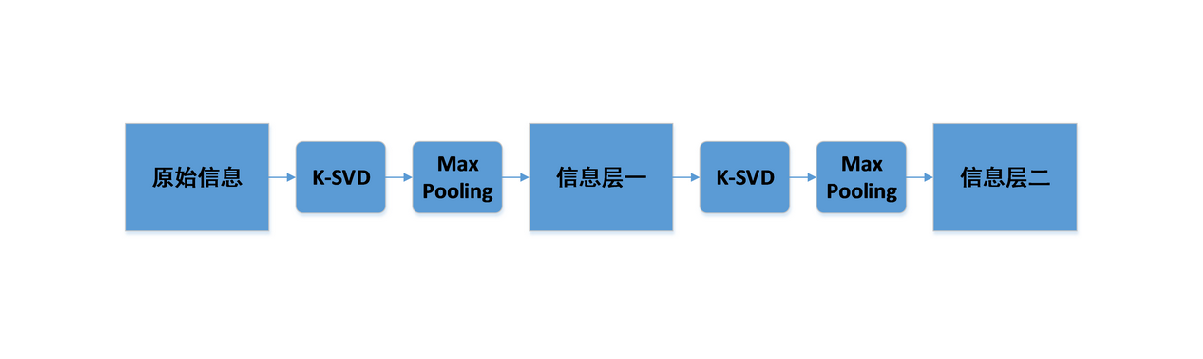
\includegraphics[width=1\textwidth]{workflow_HMP}
  \caption{分层匹配追踪的工作流}
  \label{fig:workflow_HMP}
\end{figure}

分层匹配追踪(HMP)~\inlinecite{bo2011hierarchical} 的中心概念是自动地学习低层和中层的特征,而不是使用人工选择的特征,例如SIFT~\inlinecite{ng2003sift} 等。HMP从原始数据中学习到一组稀疏字典,并使用这些字典给数据分层地编码,获得一个空间金字塔。如图~\ref{fig:workflow_HMP} 所示。具体地说,给定一组h维的观测值$Y = [y_1, ..., y_n] \in R^{h\times n}$,K-SVD的学习目标是找到一组字典$D = [d_1, ..., d_m] \in R^{m \times n}$(这里的$d_i$可以称为过滤器),和一组稀疏编码$X = [x_1, ..., x_n] \in R^{m \times n}$,使得如下重建误差最小化:
\begin{equation}
\label{equ:ksvd_minimize}
\underset{D,X}{\min}{||Y-DX||_F^2} \qquad s.t. ~ \forall i,~ ||x_i||_0 \leq K
\end{equation}
其中$||X||_F$表示X的弗罗贝尼乌斯范数(Frobenius norm);$x_i$是$X$的一列;$||*||_0$是零范数,数值等于$x_i$中为零项的个数;$K$是稀疏级别,表示每一组数据中为零项个数的上限。因为~\ref{equ:ksvd_minimize} 中的问题是非凸的,很难给出精确解,所以在实际操作中我们采用近似解法OMP~\inlinecite{aharon2006img} 来贪心地求解。具体地说,OMP会迭代地交替执行以下两个过程,逐步逼近最终结果。
$$
\underset{X}{\min}{||Y-D^*X||_F^2}
$$
$$
\underset{X}{\min}{||Y-DX^*||_F^2}
$$

通过K-SVD的提取出来的信息,可以较好地重构出原来的图片,如图\ref{fig:ksvd_rebuild}所示。重构出的图片与原图质量相差无几,说明尽管在使用分层匹配追踪时信息的维度和结构发生了较大变化,但大部分有用信息都被保留了下来。

\begin{figure}[H] % use float package if you want it here
  \centering
  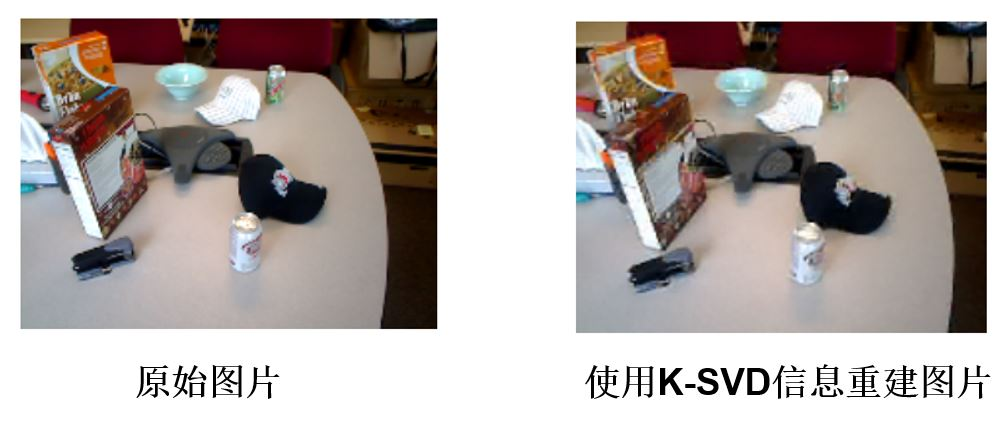
\includegraphics[width=0.9\textwidth]{ksvd_rebuild}
  \caption{K-SVD 保留信息可视化}
  \label{fig:ksvd_rebuild}
\end{figure}

如果将K-SVD学习得到的字典可视化,可以得到如图\ref{fig:ksvd_dict}所示的效果,可以看出:在深度、颜色信息之中学习到的字典(过滤器)均包含一定的有规律可循的模式,比如说边、角、点。其中RGB图片的字典含有颜色信息,而深度图片学习到的字典虽然没有颜色信息,但是边角分界处往往更加锋利清晰,这也体现了两种模态信息的互补性。

空间金字塔最大池化(Spatial pyramid max pooling)是一种高度非线性的信息处理过程,可以从局部稀疏编码中生成更高层次、更低维度的表征方式。它的结构如图~\ref{fig:maxpooling}所示~\inlinecite{yang2009linear}。
这种方法在多个层次上递归地进行最大池化。具体地说,假设最大池化的接受域为$2 \times 2$,那么第零层每个单元就代表原始数据中的一个单元,第一层每个单元代表原始数据中的四个单元,以此类推。设$U$为池化前的数据,$U$的每一列为原始数据中的邻域,$z$代表着池化之后的数据,那么最大池化可以表示为:

\begin{equation}
\begin{aligned}
z &= F(U) \\
z_j &= max\left\{|u_{1j}|, ..., |u_{Mj}|\right\}
\end{aligned}
\end{equation}

\begin{figure}[H] % use float package if you want it here
  \centering
  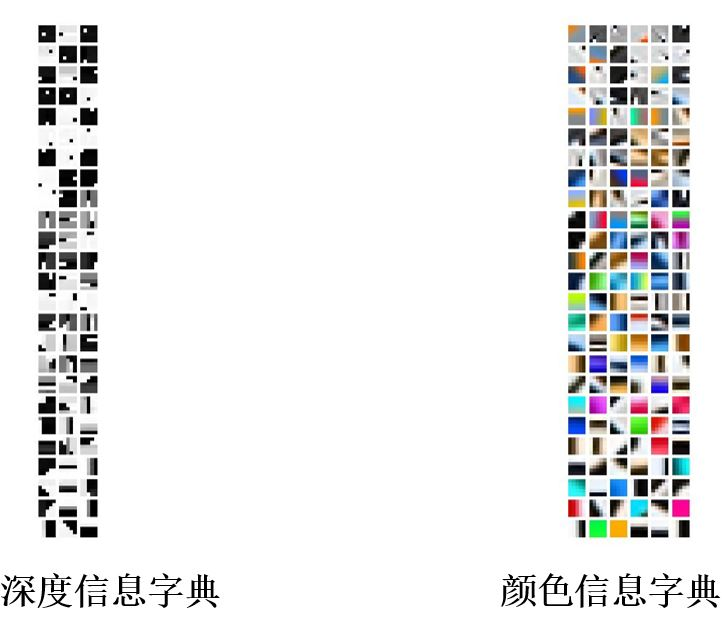
\includegraphics[width=0.65\textwidth]{ksvd_dict}
  \caption{K-SVD 字典可视化}
  \label{fig:ksvd_dict}
\end{figure}

\begin{figure}[H] % use float package if you want it here
  \centering
  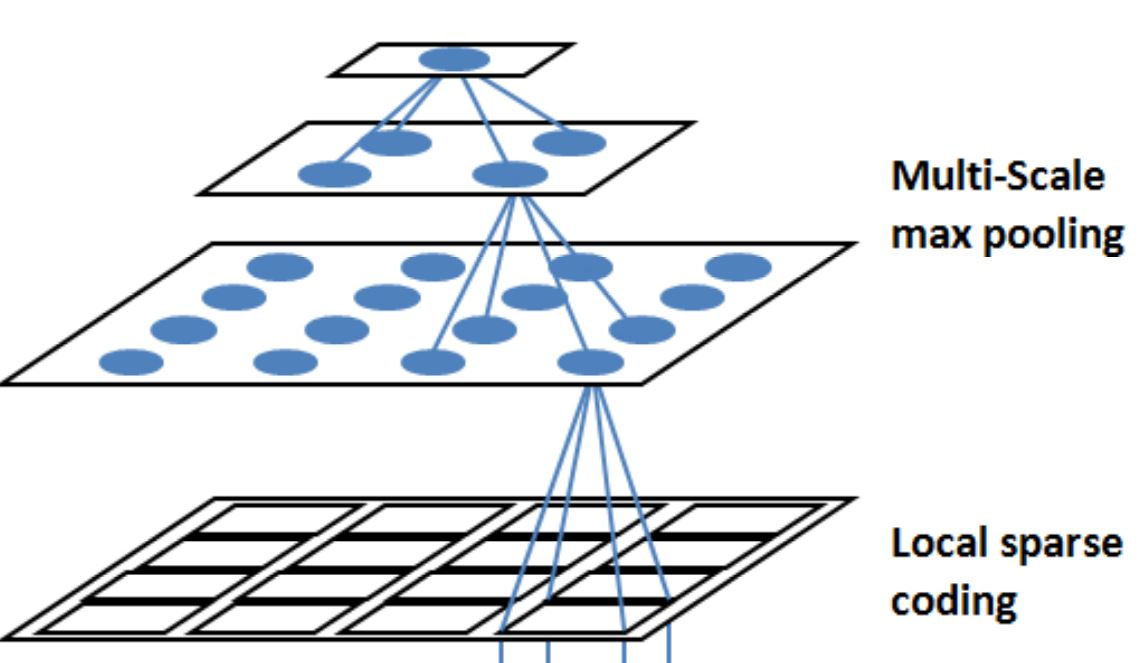
\includegraphics[width=0.8\textwidth]{maxpooling}
  \caption{空间金字塔最大池化示意图}
  \label{fig:maxpooling}
\end{figure}

具体的参数及实验效果见~\ref{sec:fStrategyExp} 小节。



\section{随机权值神经网络}
\label{sec:CRNN}

如果说分层匹配追踪是一种目的明确的监督学习(supervised learning),那么随机权值神经网络(CRNN)的信息提取过程就显得比较“随意”。在这里,我们引入CRNN作为另一种参与融合的信息提取策略,一方面是因为它可以引入一定的随机性,另一方面是因为通过神经网络的信息提取过程与传统的词袋模型(Bag of Words)具有很大不同,提取出的信息在结构上也与之有较大差别,所以可以预见CRNN与传统信息提取方法有着较大的互补性,将它们融合可以获得较大的准确率上的提升。由于一定随机性在许多人工智能策略中都可以避免陷入局部最优,提升策略表现,比如遗传算法~\inlinecite{goldberg1988genetic} 和蒙特卡洛方法~\inlinecite{metropolis1949monte} 等。所以我们也试图使用CRNN来给我们的模型引入一定的随机性。CRNN的工作流程图如图\ref{fig:workflow_CRNN} 所示。


\begin{figure}[H] % use float package if you want it here
  \centering
  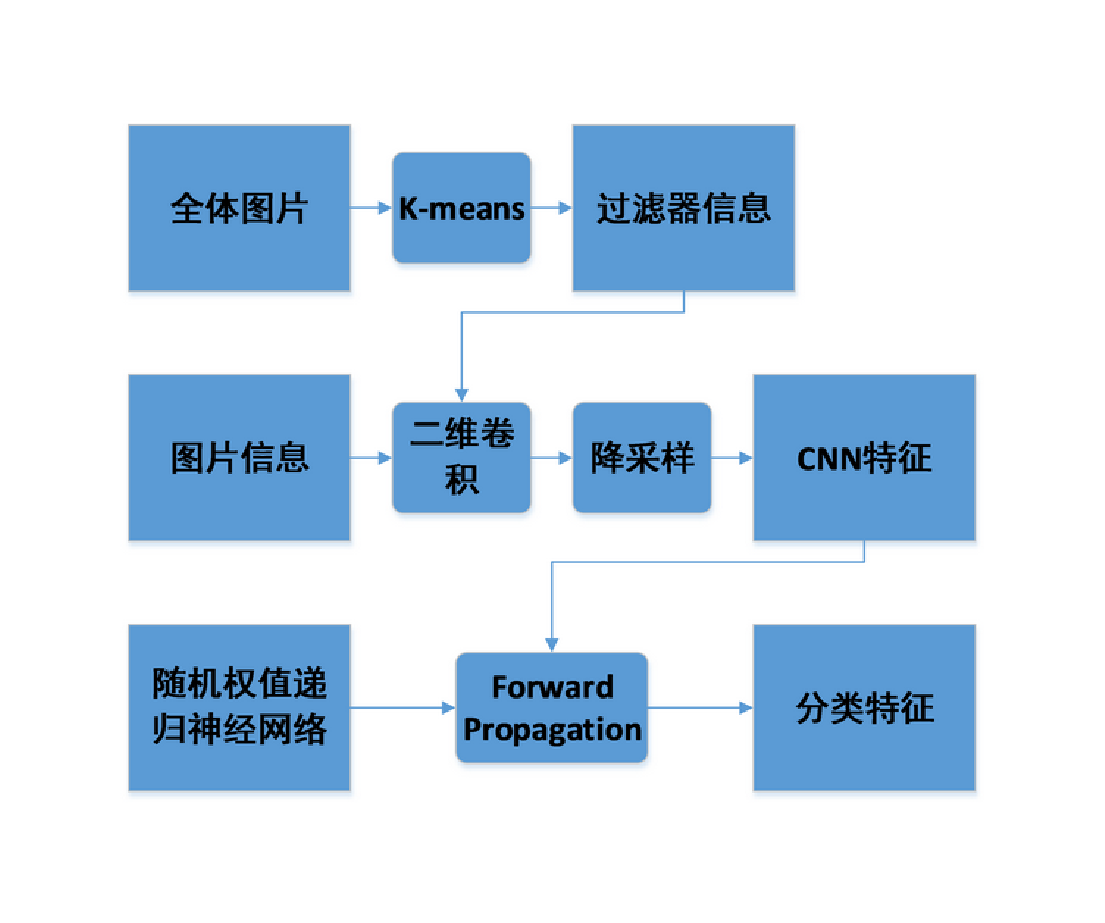
\includegraphics[width=0.95\textwidth]{workflow_CRNN}
  \caption{CRNN的的工作流}
  \label{fig:workflow_CRNN}
\end{figure}

如图\ref{fig:workflow_CRNN}所示,我们需要先得到一组过滤器,这个过滤器不一定需要在我们的训练集上学习出来,也可以在更大、更全面的数据集上预先通过K-means学习出来。
K-means的目标函数是:
\begin{equation}
\underset{S}{\min}\sum\limits_{i=1}^{k}{\sum\limits_{x \in S_i}{||x-\mu_i||^2}}
\end{equation}
其中k是K-means产生的中心的数量,S是分类信息,$\mu_i$是K-means产生的中心,$x \in S_i$说明信息x以$\mu_i$为中心。学习到的过滤器如图~\ref{fig:CNN_filters}所示。

\begin{figure}[H] % use float package if you want it here
  \centering
  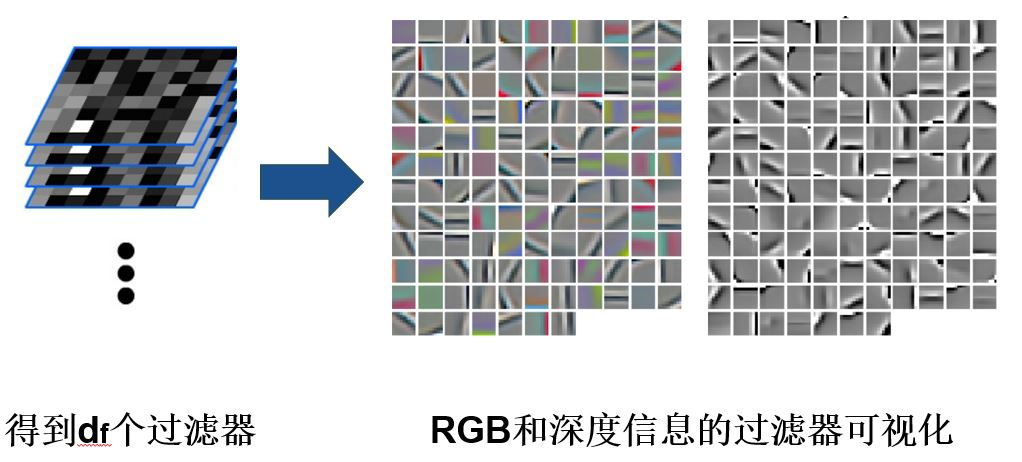
\includegraphics[width=0.95\textwidth]{CNN_filters}
  \caption{CNN的过滤器可视化}
  \label{fig:CNN_filters}
\end{figure}

然后我们使用Pretrained的过滤器信息与图片信息进行二维卷积和降采样,如图~\ref{fig:CNN_structure} 所示,以便得到图片的CNN特征。

由于我们使用一组过滤器分别与原图片卷积,所以对于每一张图片输入会得到一组CNN的模式(pattern)。通过CNN提取出的某个目标物体(一个苹果)的pattern如图~\ref{fig:CNN_feature}所示。可以看出,左边的RGB pattern含有一定的光照、纹理信息;而右边的Depth pattern则含有更加锋利明显的边界信息,这也体现了两种模态信息的互补性。

\begin{figure}[H] % use float package if you want it here
  \centering
  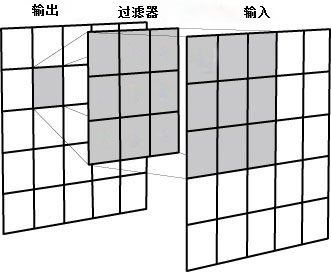
\includegraphics[width=0.8\textwidth]{CNN_structure}
  \caption{CNN的结构}
  \label{fig:CNN_structure}
\end{figure}

\begin{figure}[H] % use float package if you want it here
  \centering
  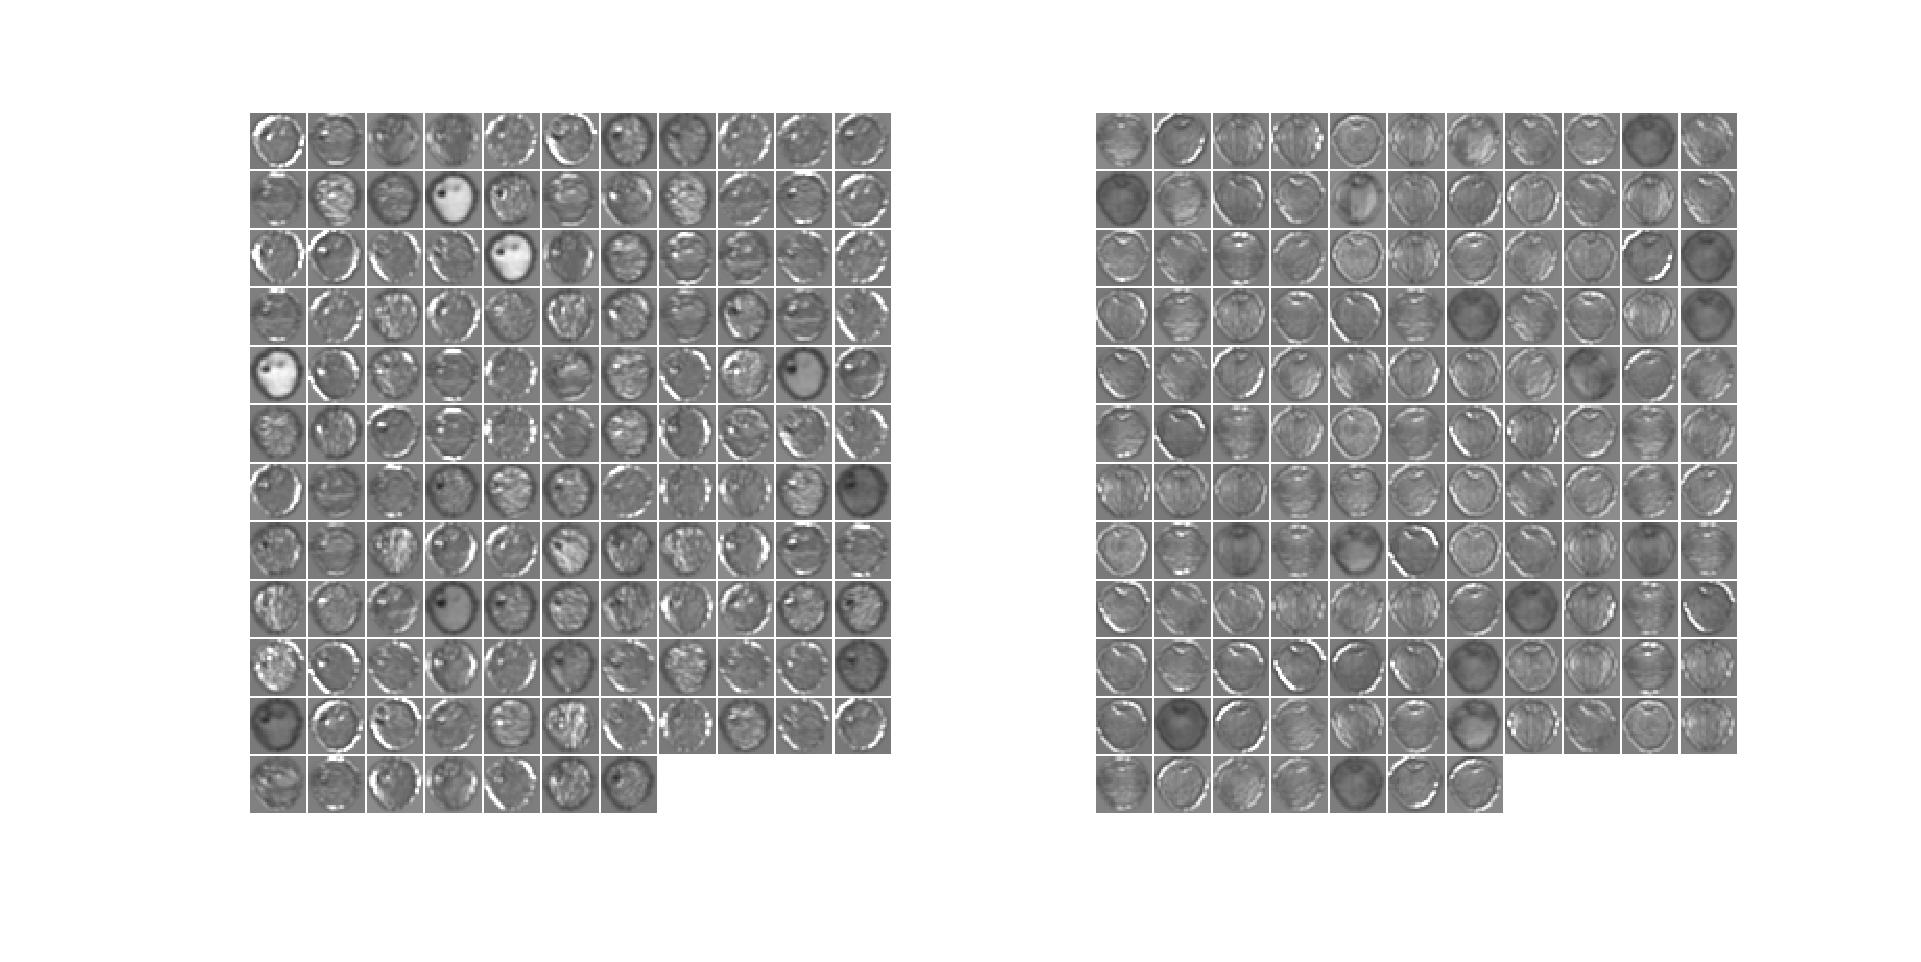
\includegraphics[width=1.1\textwidth]{CNN_feature}
  \caption{CNN所提取出的模式(左为RGB patter,右为Depth patter)}
  \label{fig:CNN_feature}
\end{figure}

然后我们将得到的CNN模式输入一组递归神经网络(RNN)。注意,这里我们虽然使用了神经网络,但是由于其权值是随机产生的,不会在信息提取的过程中改变,并且我们只使用前向传递(forward propagation)而不使用后向传递(back propagation),所以这并不是一个监督学习的过程,而是一个非监督(unsupervised)的信息提取过程。在这一步中我们对于每一层的每个接受域(相近的指定大小的区域)中的数值施加一个变换,得到一个数值作为更高层相应单元中的数值。具体地说:
\begin{equation}
\label{equ:RNN}
x_i^h = f(X_i^{h-1})
\end{equation}
其中,$x_i^h$代表h层的单元i的数值,$X_i^{h-1}$代表h层的单元i在h-1层对应的接受域内的数值矩阵。可以看出,RNN其实是空间金字塔最大池化(Spatial pyramid max pooling)的推广——将~\ref{equ:RNN} 式中的$f()$函数设置为取$max$就是空间金字塔最大池化。不过我们在分类时往往只使用上层的信息。RNN的工作示意图如图~\ref{fig:RNN_structure} 所示。


\begin{figure}[H] % use float package if you want it here
  \centering
  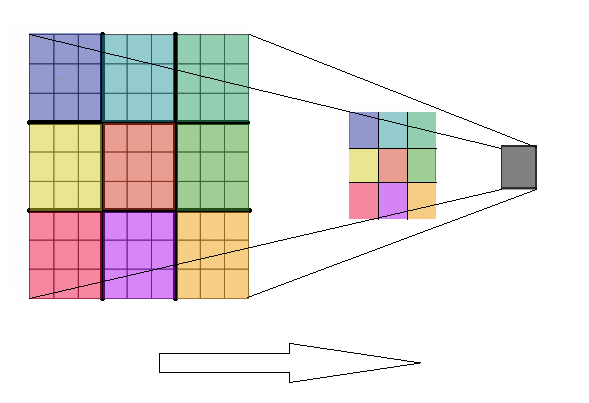
\includegraphics[width=0.95\textwidth]{RNN_structure}
  \caption{RNN工作示意图}
  \label{fig:RNN_structure}
\end{figure}

具体的参数及实验效果见~\ref{sec:fStrategyExp} 小节。


\section{多模态融合策略}
\label{sec:fStrategy}

\subsection{特征层融合}
\label{subsec:fInMethod}

对于同一方法内,不同模态间的信息融合,我们倾向于使用特征层的融合策略。因为正如前文所述,RGB信息和深度信息有着天然的互补性,而这些互补性在特征层体现得最明显。如果我们先分别利用颜色信息和深度信息得到一个分类的估计值,这样虽然具有了一定的语义信息,也可以从贝叶斯的角度来增大最终分类的准确率,但是这样就不能完全挖掘颜色和深度信息之间的联系与互补性。在实验中我们尝试了使用决策层的融合策略和特征层的融合策略,发现对于同一方法内的融合,在特征层的操作确实在大多数情况下会取得更好的结果。

具体地说,我们使用连接作为特征层融合的方法:
\begin{equation}
\label{equ:feature_level}
X_{feature} = [X_{RGB}, X_{D}]
\end{equation}
其中$X_{feature}$是特征层融合得到的信息,$X_{RGB}$是颜色图片提取出的信息,$X_{D}$是深度图片提取出的信息。

\subsection{决策层融合}
\label{subsec:fBetweenMethod}

而对于不同方法之间的信息融合,我们更倾向于使用决策层的融合策略。原因如下:
\begin{enumerate}
\item 由于方法的不同,各组特征之间维度差异较大,在特征层难以权衡各个方法在总体决策中占的权重,维数越高的信息在特征层融合之后占总体决策权重就会越大。
\item 各组特征结构差异较大,如果使用特征层融合,难以捕捉其中的联系。相反,有可能造成过拟合。
\item 由于在特征层融合之后特征的维度往往比较高,对于接下来的决策步骤中的计算资源要求也较高。而采用决策层融合的策略可以分而治之,将特征压缩为带有语义的信息再做处理。
\end{enumerate}

在实验中,由于需要两个分类器带权投票,我们需要能够产生分类自信度的分类器,所以优先试验了贝叶斯分类器。但是发现贝叶斯分类器在信息矩阵维数较高时计算过于缓慢,且效果也不如SVM。所以我们决定使用SVM分类器来进行分类决策。不过因为原生的SVM只能够产生分类结果,而不能产生分类自信度,为了实现决策级的信息融合,我们使用Sigmoid-Softmax方法将SVM的决策值转化为自信度估计,如~\ref{equ:sigmoid_softmax} 式所示。

\begin{equation}
\label{equ:sigmoid_softmax}
P(C_j|I_i) = \frac{Sigmoid(dec\_value_{ij})}{\underset{k}{\sum}{Sigmoid(dec\_value_{ik})}}
\end{equation}

最终,我们在使用~\ref{equ:sigmoid_softmax} 式得出两种方法各自的分类自信度之后投票决定最终输出结果。实验证明,我们提出的融合策略可以有效地捕捉方法间的信息互补性,使得最终分类结果有所提升。整体融合策略的框架如图~\ref{fig:workflow_fstrategy} 所示。

\begin{figure}[H] % use float package if you want it here
  \centering
  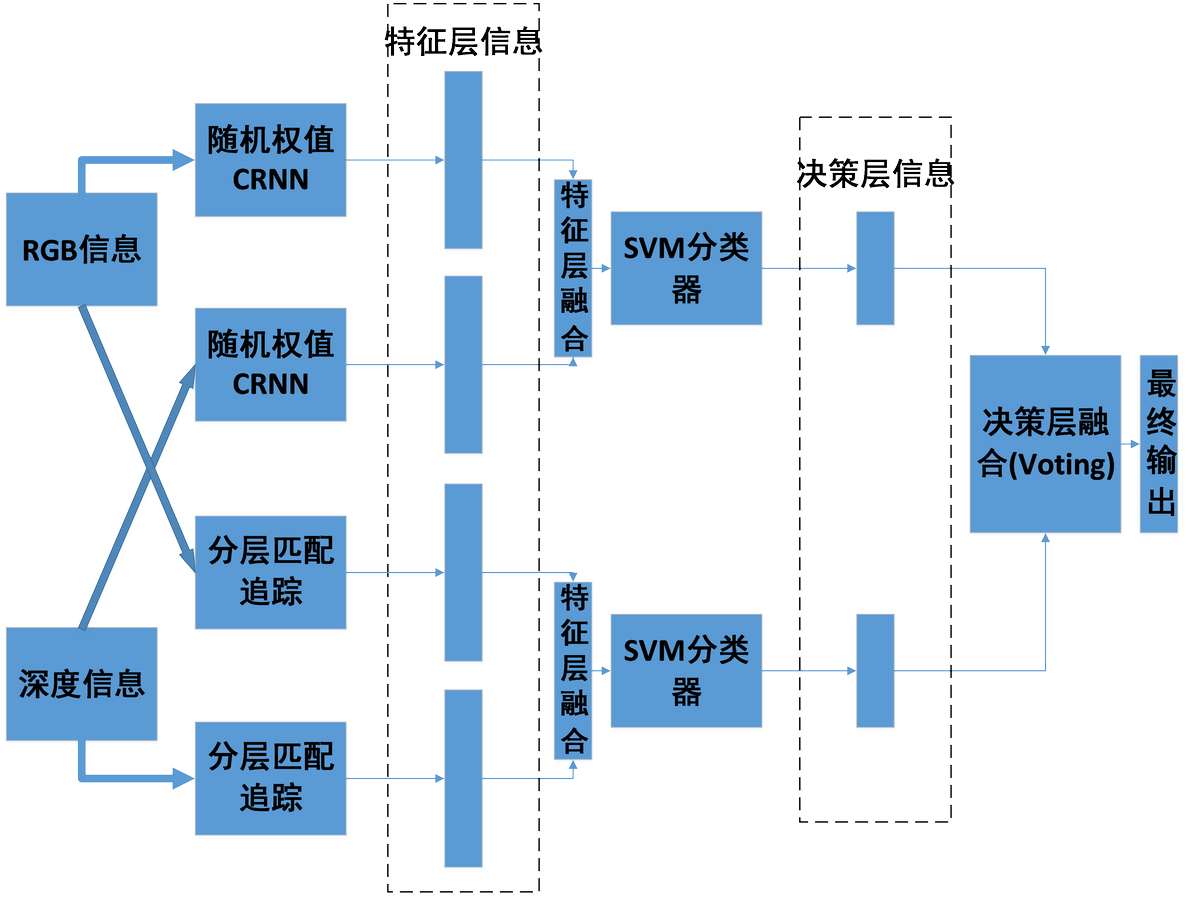
\includegraphics[width=0.95\textwidth]{workflow_fstrategy}
  \caption{整体融合策略的框架}
  \label{fig:workflow_fstrategy}
\end{figure}

具体的参数及实验效果见~\ref{sec:fStrategyExp} 小节。


\section{试验验证}
\label{sec:fStrategyExp}

\subsection{试验综述}

我们选用了上文中提到的华盛顿大学RGB-D数据集~\inlinecite{lai2011large} 作为我们的训练集。此数据集包含分别属于51个类别的日常用品的300个物体实例,如图~\ref{fig:washington}所示。总共包含超过20万组匹配的RGB-D图片,在实验中我们为了与~\inlinecite{lai2011large} 的baseline对比,所以选用了其中的41877组RGB-D信息。

\begin{figure}[H] % use float package if you want it here
  \centering
  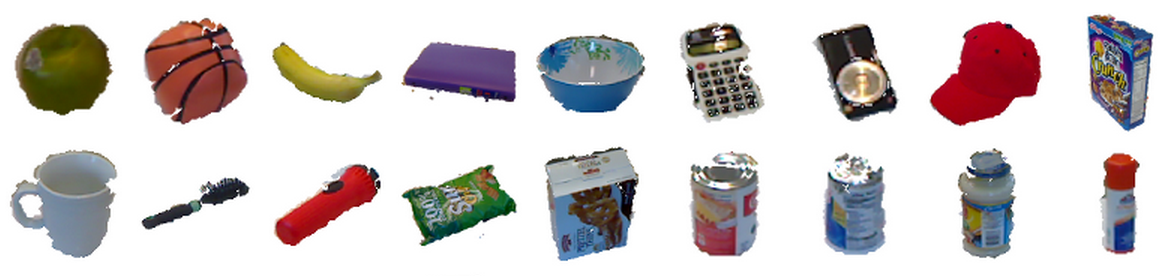
\includegraphics[width=0.95\textwidth]{washington}
  \caption{华盛顿RGB-D数据集}
  \label{fig:washington}
\end{figure}

在本节中我们对颜色信息和深度信息分别用CRNN和HMP两种方法进行分类,然后将两种模态在不同层次融合起来进行分类,以观察模态间融合的效果提升。然后我们为了探究不同模态之间的互补性,对比了两种模态的混淆矩阵,并对其中典型的例子进行了探讨。最后我们统一使用RGB-D信息,用两种方法进行分类并尝试在不同层次进行融合,以探究方法融合的效果。其中SVM分类器的实现我们选择使用 liblinear~\inlinecite{REF08a} 。

\subsection{试验参数}

对于分层匹配追踪,我们需要在两个层次上设置相应的参数。

第一层。从1000000个$5 \times 5$的深度图片样本中学习出75组稀疏度为5的灰度字典和深度字典;从1000000个$5 \times 5 \times 3$的RGB图片样本中学习出150组稀疏度为5的颜色字典和曲面法线字典。接下来我们使用上述字典,使用OMP算出原图对应的稀疏编码,并使用空间金字塔最大池化的方法产生$16 \times 16$,$4 \times 4$,$2 \times 2$,$1 \times 1$的信息,将它们拼接在一起压缩成一维,作为第一层的输出特征。

第二层。在第一层输出的基础上从1000000个$5 \times 5$的深度图片和RGB图片产生的输出特征中学习出1000组稀疏度为10的灰度字典、深度字典、颜色字典和曲面法线字典。接下来我们使用上述字典,使用OMP算出第一层输出对应的稀疏编码,并使用空间金字塔最大池化的方法产生$3 \times 3$,$2 \times 2$,$1 \times 1$的分割信息,将它们拼接在一起压缩成一维,得到总共$4(channel) \times 1000(dict) \times (3 \times 3 + 2 \times 2 + 1 \times 1) = 54000$维向量,作为第一层的输出特征(其中RGB和深度信息分别为28000维)。因为第一层信息维度过高,所以在实验中我们只使用第二层的信息。

对于CRNN,我们同样需要在两个层次上设置参数。

CNN层。学习出128个过滤器,分别和RGB和深度图片卷积之后降采样得到$27 \times 27$的图片块,所以对于每一张RGB或深度图片分别可以得到$128 \times 27 \times 27$的图片块(见图片~\ref{fig:CNN_feature})。

RNN层。利用CNN层得到的维度为$128 \times 27 \times 27$的图片块,将每一个过滤器对应的$27 \times 27$的图片块分别通过128个随机产生的RNN,每个RNN得到 $1 \times 1$ 维特征。所以最终我们得到每张RGB和深度图片对应的信息分别为$128 \times 128 = 16384$维,总共有32768维输出信息。

\subsection{试验结果}

在实验中,我们采用以上的参数设置,得到如下实验结果:

\begin{table}[htbp]
  \centering
  \caption{模态间融合实验结果}
  \label{tab:fStrategyResult1}
  \begin{minipage}[t]{0.8\textwidth} 
    \begin{tabularx}{\linewidth}{|l|X|X|X|X|}
      \hline
 \multirow{2}*{\diagbox[width=5em]{方法}{模态}} & \multirow{2}*{RGB} & \multirow{2}*{Depth} & \multicolumn{2}{c|}{RGB \& Depth}\\\cline{4-5}
      & & &特征融合$^{*}$&决策融合$^{**}$ \\ \hline
      CRNN      & $81.7 \pm 1.4$ & $78.9 \pm 1.6$ & $\boldsymbol{87.6 \pm 1.2}$ & $87.3 \pm 1.1$ \\
      HMP       & $75.8 \pm 3.4$ & $78.4 \pm 1.9$ & $85.4 \pm 2.6$ & $\boldsymbol{86.3 \pm 2.1}$ \\
      决策融合  & $83.1 \pm 2.6$ & $82.5 \pm 1.9$ & $\boldsymbol{89.6 \pm 2.1}$ & $89.1 \pm 1.8$ \\ \hline
    \end{tabularx}\\[2pt]
    \footnotesize
    *:使用~\ref{equ:feature_level} 式\\
    **:使用~\ref{equ:sigmoid_softmax} 式
  \end{minipage}
\end{table}

通过表~\ref{tab:fStrategyResult1} 我们可以看出,多模态信息融合可以明显提升分类准确率。下面我们以匹配追踪为例,来探究两种模态的信息互补性。两种模态信息分类的混淆矩阵(Confusion Matrix)如图~\ref{fig:confusion_matrix} 所示。混淆矩阵~\inlinecite{townsend1971theoretical} 是在监督学习中对于分类结果的可视化,其每一列表示了一个预测类别;其每一行表示了一个真实类别,一个数据实例属于第i行第j列当且仅当此实例数据第i类,被分类模型分到第j类。颜色越深的区域中含分类实例越多,所以理想化的混淆矩阵应该是对角矩阵。通过对两者混淆矩阵的比较可以看出,它们是有一定的互补性的。例如图片~\ref{fig:instance} 所示,如果只使用深度信息,容易将peach分类为sponge,如果只使用颜色信息,又容易将sponge分类为rubber eraser。而将两种信息结合起来之后,上述三种物品均可以得到较好分类。

\begin{figure}[H] % use float package if you want it here
  \centering
  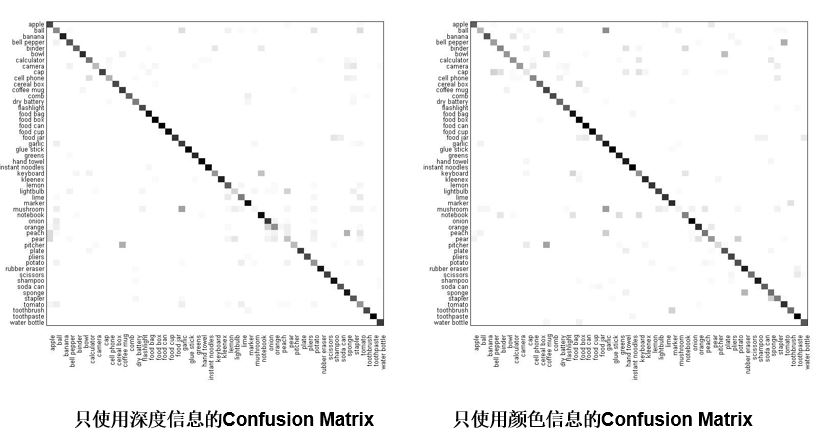
\includegraphics[width=0.95\textwidth]{confusion_matrix}
  \caption{两种模态信息分类的混淆矩阵}
  \label{fig:confusion_matrix}
\end{figure}

\begin{figure}[H] % use float package if you want it here
  \centering
  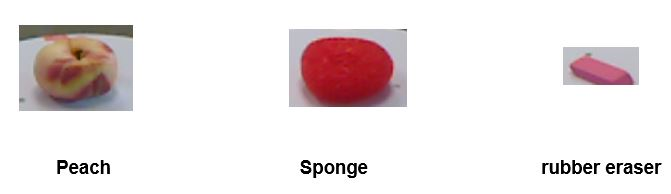
\includegraphics[width=0.95\textwidth]{instance}
  \caption{分类效果举例}
  \label{fig:instance}
\end{figure}

\begin{table}[htbp]
  \centering
  \caption{方法间融合实验结果}
  \label{tab:fStrategyResult2}
  \begin{minipage}[t]{0.8\textwidth} 
    \begin{tabularx}{\linewidth}{|X|X|X|X|}
      \hline
      CRNN & HMP & CRNN \& HMP 特征融合$^{*}$ & CRNN \& HMP 决策融合$^{**}$ \\ \hline
      $87.6 \pm 1.2$ & $85.4 \pm 2.6$ & $88.7 \pm 2.0$ & $\boldsymbol{89.6 \pm 2.1}$ \\ \hline
    \end{tabularx}\\[2pt]
    \footnotesize
    本表展示的均是使用RGB-D信息得到的结果。\\
    *:使用~\ref{equ:feature_level} 式\\
    **:使用~\ref{equ:sigmoid_softmax} 式
  \end{minipage}
\end{table}

接下来我们使用RGB-D信息,探究两种信息提取方法之间的融合策略。得到结果如表~\ref{tab:fStrategyResult2} 所示。
可以看出,不论是模态间还是方法间的信息融合都可以明显提高分类的准确率。而且正如我们预测的一样,在方法间采用决策层的融合可以更好的提升效果。我们在图~\ref{fig:workflow_fstrategy} 中提出的融合模型,可以综合使用图~\ref{fig:workflow_HMP} 和图~\ref{fig:workflow_CRNN} 中的方法,并得到有效的效果提升。